\documentclass[]{article}

\usepackage{caption,subcaption,graphicx,float,url,amsmath,amssymb,amsthm,tocloft,cancel,thmtools,gensymb,braket,bm}
\usepackage[toc,nonumberlist]{glossaries}
\usepackage{glossaries-extra}
\usepackage[toc,page]{appendix}

\newcommand\numberthis{\addtocounter{equation}{1}\tag{\theequation}}

\newtheorem{thm}{Theorem}
\newtheorem{defn}[thm]{Definition}
\newtheorem{cor}[thm]{Corollary}
\newtheorem{lemma}[thm]{Lemma}
\graphicspath{{figs/}}
\widowpenalty10000
\clubpenalty10000
\setcounter{tocdepth}{2}

%opening
\title{Theoretical Minimum\\General Relativity}
\author{}

\begin{document}

\maketitle

\begin{abstract}
	These are my notes for the \emph{General Rrlativity}\cite{susskind2012general} lectures from Leonard Susskind's \emph{Theoretical Minimum} series\cite{susskind2007theoretical}.
\end{abstract}

\tableofcontents
\listoffigures
\listoftables
\listoftheorems

\section{The equivalence principle and tensor analysis}

LS begins where Einstein started. Einstein started with the simplest things and deduced far racing conclusions.

\subsection{The equivalence principle}

This is the principle that gravity is, in some sense, the same as acceleration.

If we are in an accelerated frame of reference, an elevator moving up or down say, we feel a gravitational field. Children know that.

Figure \ref{fig:gr-1-elevator} depicts an elevator. Assuming we know the laws of physics in the $z$ frame, surely we can figure then out in $z^\prime$.

\begin{figure}[H]
	\caption[Moving Elevator]{Moving Elevator: there are two coordinate systems, $z$ and $z^\prime$, and $L(t)$ alows us to pass from one to the other.}\label{fig:gr-1-elevator}
	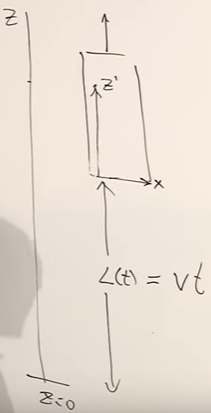
\includegraphics{gr-1-elevator}
\end{figure}

\subsection{Tensor analysis}

\section{Tensor mathematics}

TBP

\section{Flatness \& curvature}

TBP

\section{Geodesics \& gravity}

TBP

\section{Metric for a gravitational field}

TBP

\section{Black holes}

TBP

\section{Falling into a black hole}

TBP

\section{Formation of a black hole}

TBP

\section{Einstein field equations}

TBP

\section{Gravity Waves}

TBP

\bibliographystyle{unsrt}
\addcontentsline{toc}{section}{Bibliography}
\raggedright
\bibliography{tm}

\end{document}
